\chapter{MÉTODOS DE AMOSTRAGEM}

\textbf{\textit{“A amostragem é a mãe da precisão, pois nos permite fazer grandes descobertas a partir de pequenas porções de dados.” – \textbf{William Sealy Gosset}}} \vskip0.3cm

\section{Introdução}

O objetivo de todo projeto de pesquisa é, a partir do estudo de uma amostra, fazer inferências sobre uma determinada população. Logo, para que a inferência estatística seja válida, é necessário que a amostra seja representativa da população de onde foi retirada, de maneira que os resultados encontrados sejam os mais fidedignos possíveis (CALLEGARI-JAQUES, 2003). 
\vskip0.3cm

Assim, é necessário que o autor do projeto atente para fatores cruciais, tais como o método de amostragem e o cálculo do tamanho amostral. Amostras mal selecionadas ou de tamanho inadequado comprometem o resultado da pesquisa, uma vez que não representam fielmente a população (DAWSON, 2003). \vskip0.3cm

Nesse sentido, o cálculo do tamanho amostral tem sido um dos maiores desafios para pesquisadores. Nem sempre os métodos para esse cálculo se apresentam de maneira simples e compreensível, o que gera ansiedade e dúvidas no processo experimental (BEIGUELMAN, 2002). \vskip0.3cm

Para Silva (2004), os levantamentos por amostragem têm a finalidade de produzir "instantâneos" das realidades estudadas e reúnem as seguintes características operacionais:

\begin{enumerate}
    \item[{i)}] Aplicam-se a conjuntos reais e finitos, denominados \textbf{população de estudo}.
    \item[{ii)}] Os elementos podem ser seres humanos, animais, árvores, prontuários, domicílios, áreas ou objetos.
    \item[{iii)}] As características (atributos) são observadas em cada elemento e agregadas por meio de medidas estatísticas chamadas \textbf{parâmetros} ou valores populacionais.
    \item[{iv)}] Os dados são coletados em amostras, e as medidas calculadas (\textbf{estimativas}) tornam-se a informação disponível para os valores populacionais desconhecidos.
\end{enumerate}

De acordo com Silva (2004), os levantamentos podem ter finalidade \textbf{descritiva}, limitando-se a estimar frequências, médias e variâncias. Outros, denominados \textbf{analíticos ou investigações}, buscam detectar relações entre características, aumentando o poder explicativo sobre o objeto pesquisado. \vskip0.3cm

As técnicas de amostragem são classificadas em duas categorias principais: \textbf{Probabilísticas} e \textbf{Não Probabilísticas}.
\vskip0.3cm

\textbf{Amostragem Probabilística (Casual):} Ocorre quando se conhece a probabilidade (diferente de zero) de cada elemento da população pertencer à amostra. Exige que a população seja finita e acessível. Exemplos: aleatória simples, sistemática, estratificada e por conglomerados (MATTAR, 2001). 

\vskip0.3cm

\textbf{Amostragem Não Probabilística (Não Casual):} Nem todos os elementos têm probabilidade conhecida de participar. É utilizada quando o acesso à população é restrito ou o material é contínuo. Exemplos comuns incluem a amostragem por \textbf{conveniência}, \textbf{intencional}, \textbf{por quotas} e a técnica de \textbf{bola de neve (snowball)}, onde um participante indica outro (MATTAR, 2001). \vskip0.3cm

\subsection{Fatores que Afetam o Tamanho da Amostra} 

O tamanho da amostra depende de fatores que influenciam a precisão e a confiabilidade dos resultados:

\begin{itemize}
    \item \textbf{Objetivo do Estudo}: Estudos descritivos podem exigir tamanhos diferentes de estudos comparativos.
    \item \textbf{Variabilidade do Fenômeno}: Quanto maior a dispersão (variância) dos dados na população, maior deve ser a amostra.
    \item \textbf{Nível de Confiança (Erro Alfa $\alpha$)}: É a probabilidade de rejeitar a hipótese nula quando ela é verdadeira (falso-positivo). Comumente fixado em 5\%. Quanto menor o erro aceitável, maior a amostra.
    \item \textbf{Poder do Teste ($1-\beta$)}: Probabilidade de detectar um efeito real (evitar falso-negativos). Geralmente fixado entre 80\% e 90\%. 
    \item \textbf{Tamanho do Efeito}: Refere-se à menor diferença que o pesquisador deseja detectar. Diferenças muito pequenas exigem amostras significativamente maiores.
    \item \textbf{Tamanho da População}: Relevante para populações pequenas (finitas). Em populações muito grandes, o impacto no cálculo é minimizado.
\end{itemize}

\begin{table}[h]
\centering
\small
\caption{Diferenças entre Amostragem Estratificada e por Conglomerados}
\begin{tabular}{|l|p{4.5cm}|p{4.5cm}|}
\hline
\rowcolor[gray]{0.9} \textbf{Característica} & \textbf{Estratificada} & \textbf{Conglomerados} \\ \hline
\textbf{Homogeneidade} & Interna ao grupo (estrato) & Externa (entre os grupos) \\ \hline
\textbf{Heterogeneidade} & Externa (entre estratos) & Interna (dentro do grupo) \\ \hline
\textbf{Seleção} & Elementos de todos os estratos & Sorteio de grupos inteiros \\ \hline
\textbf{Principal Objetivo} & Aumentar a precisão & Reduzir custos e logística \\ \hline
\end{tabular}
\end{table}
%-------------------------------------------------------------------------------------------%

\newpage
\subsection{Procedimentos Amostrais Iniciais}

O cálculo do tamanho amostral impõe ao pesquisador a especificação de um valor predefinido para o \textbf{erro amostral} (margem de erro). Este valor deve ser interpretado em termos probabilísticos: mesmo uma amostra suficientemente grande não garante que suas características sejam idênticas às da população, uma vez que sempre existe a probabilidade de a randomização gerar uma amostra atípica. \vskip0.3cm

A margem de erro ($\epsilon_0$) exprime o valor máximo de variação que o pes\-qui\-sa\-dor admite na estimativa dos parâmetros estudados em relação ao valor real da população (FONTELLES et al., 2009). \vskip0.3cm

Inicia-se com a análise da situação em que não se conhece o tamanho da população ($N$). Nesse caso, o tamanho mínimo da amostra aleatória simples pode ser determinado através de $n_{0}$, considerado uma primeira aproximação, dado por:

\begin{equation}\label{eq:nzero_infinito}
    n_{0}= \frac{1}{(\epsilon_{0})^2}
\end{equation}

Onde $\epsilon_{0}$ é o erro amostral máximo tolerável.
\vskip0.3cm

A expressão acima mantém fixo o nível de confiança de 95\% e a variância populacional no cenário de maior heterogeneidade ($p = 0,5$). A fixação da proporção populacional em 0,5 (ou 50\%) deve-se ao fato de ser esta a situação de maior incerteza; qualquer outro valor de proporção resultaria em um tamanho de amostra menor. \vskip0.3cm

Essa abordagem é indicada para três situações:
\begin{enumerate}
    \item Quando não se conhece a proporção do evento na população.
    \item Quando estudos preliminares indicam que a proporção é próxima de 0,5.
    \item Quando o estudo analisa diversos eventos simultaneamente, sem estimativas prévias para todos eles.
\end{enumerate}

\newpage
A Tabela \ref{tab:amostras} exemplifica a relação inversa entre o erro tolerável e o tamanho da amostra inicial ($n_0$).

\begin{table}[!htb]
    \centering
    \caption{Tamanho de amostra ($n_{0}$) em função do erro amostral tolerável ($\epsilon_0$).}
    \label{tab:amostras}
    \vspace{0.2cm}
    \begin{tabular}{c|c}
    \hline\hline
    \textbf{Erro Amostral} $(\epsilon_{0})$ & \textbf{Tamanho Amostral} $(n_{0})$ \\
    \hline\hline
    1,0\% (0,010)    &  10.000 \\
    2,0\% (0,020)    &  2.500  \\
    2,5\% (0,025)    &  1.600  \\
    3,0\% (0,030)    &  1.111  \\
    4,0\% (0,040)    &  625    \\
    5,0\% (0,050)    &  400    \\
    \hline\hline
    \end{tabular}
\end{table}

Como observado, quanto maior a precisão desejada (menor o erro), significativamente maior será o esforço amostral necessário. Por exemplo, reduzir o erro de 5\% para 2,5\% exige quadruplicar o tamanho da amostra (de 400 para 1.600 indivíduos).
\vskip0.3cm

\subsubsection{Correção para Populações Finitas}

Quando o tamanho da população ($N$) é conhecido, deve-se ajustar o cálculo de $n_{0}$ para obter o tamanho amostral final ($n$), utilizando a fórmula de correção:

\begin{equation}\label{eq:n_final}
n = \frac{N \cdot n_{0}}{N + n_{0}}
\end{equation}

\textbf{Exemplo Prático:}
Rocha (2013) realizou um levantamento na Delegacia de Crimes contra a Mulher de Macapá (AP). Do universo de ocorrências, identificou-se $N = 994$ casos relativos à violência conjugal. Para extrair uma amostra representativa com erro tolerável de 5\% ($\epsilon_0 = 0,05$): \vskip0.3cm

\newpage
1. Cálculo do tamanho inicial:
\begin{equation}
    n_{0}= \frac{1}{(0,05)^2} = 400
\end{equation}

2. Ajuste para a população finita ($N = 994$):
\begin{equation}
    n = \frac{994 \times 400}{994 + 400} = \frac{397.600}{1.394} \approx 285
\end{equation}

Assim, uma amostra de \textbf{285 ocorrências} é estatisticamente representativa para essa população, respeitando a margem de erro estabelecida.

%--------------------------------------------------------------------------------------------%
\section{Amostragem Probabilística}

Os principais métodos de amostragem probabilística são: Aleatória Simples, Sistemática, Estratificada e por Conglomerados.

\subsection{Amostragem Aleatória Simples (AAS)}

Este tipo de amostragem, também chamada de Casual Simples ou Randômica, baseia-se em um processo estritamente aleatório, no qual todas as unidades amostrais são selecionadas com igual probabilidade ($1/N$), sendo $N$ o número total de unidades que compõem a população (QUEIROZ, 2012).
\vskip0.3cm

A amostragem aleatória simples pode ser realizada:
\begin{itemize}
    \item \textbf{Com Reposição:} Cada elemento pode ser selecionado mais de uma vez para compor a amostra.
    \item \textbf{Sem Reposição:} Cada elemento é selecionado uma única vez.
\end{itemize}
\vskip0.3cm

Na amostragem simples ao acaso sem reposição, as unidades são selecionadas independentemente, e o número de amostras possíveis (\textit{nap}) de tamanho $n$ é dado pela combinação:

\begin{equation}\label{nap}
    nap = \binom{N}{n} = \frac{N!}{n!(N-n)!}
\end{equation}

A AAS é um processo congruente, ou seja, quando $n=N$, as estimativas coincidem com os valores populacionais. É recomendada para populações homogêneas com relação às variáveis de interesse e que possuam fácil acessibilidade.

\subsection{Amostragem Estratificada (AE)}

Muitas vezes a população se divide em subpopulações ou estratos, sendo razoável supor que, em cada estrato, a variável de interesse apresente um comportamento distinto. Por outro lado, assume-se que o comportamento é razoavelmente homogêneo dentro de cada estrato. \vskip0.3cm

Se o sorteio for realizado sem considerar a existência desses estratos, pode ocorrer uma sub-representação de determinados grupos, o que influenciará negativamente os resultados. Para evitar esse viés, adota-se a amostragem estratificada, que consiste em predeterminar quantos elementos da amostra serão retirados de cada estrato.
\vskip0.3cm

As formas mais comuns de estratificação são:
\begin{itemize}
    \item \textbf{Uniforme:} Sorteia-se um número igual de elementos em cada estrato.
    \item \textbf{Proporcional:} O número de elementos sorteados em cada estrato é proporcional ao tamanho do estrato na população.
\end{itemize}

\begin{figure}[htbp]
    \centering
    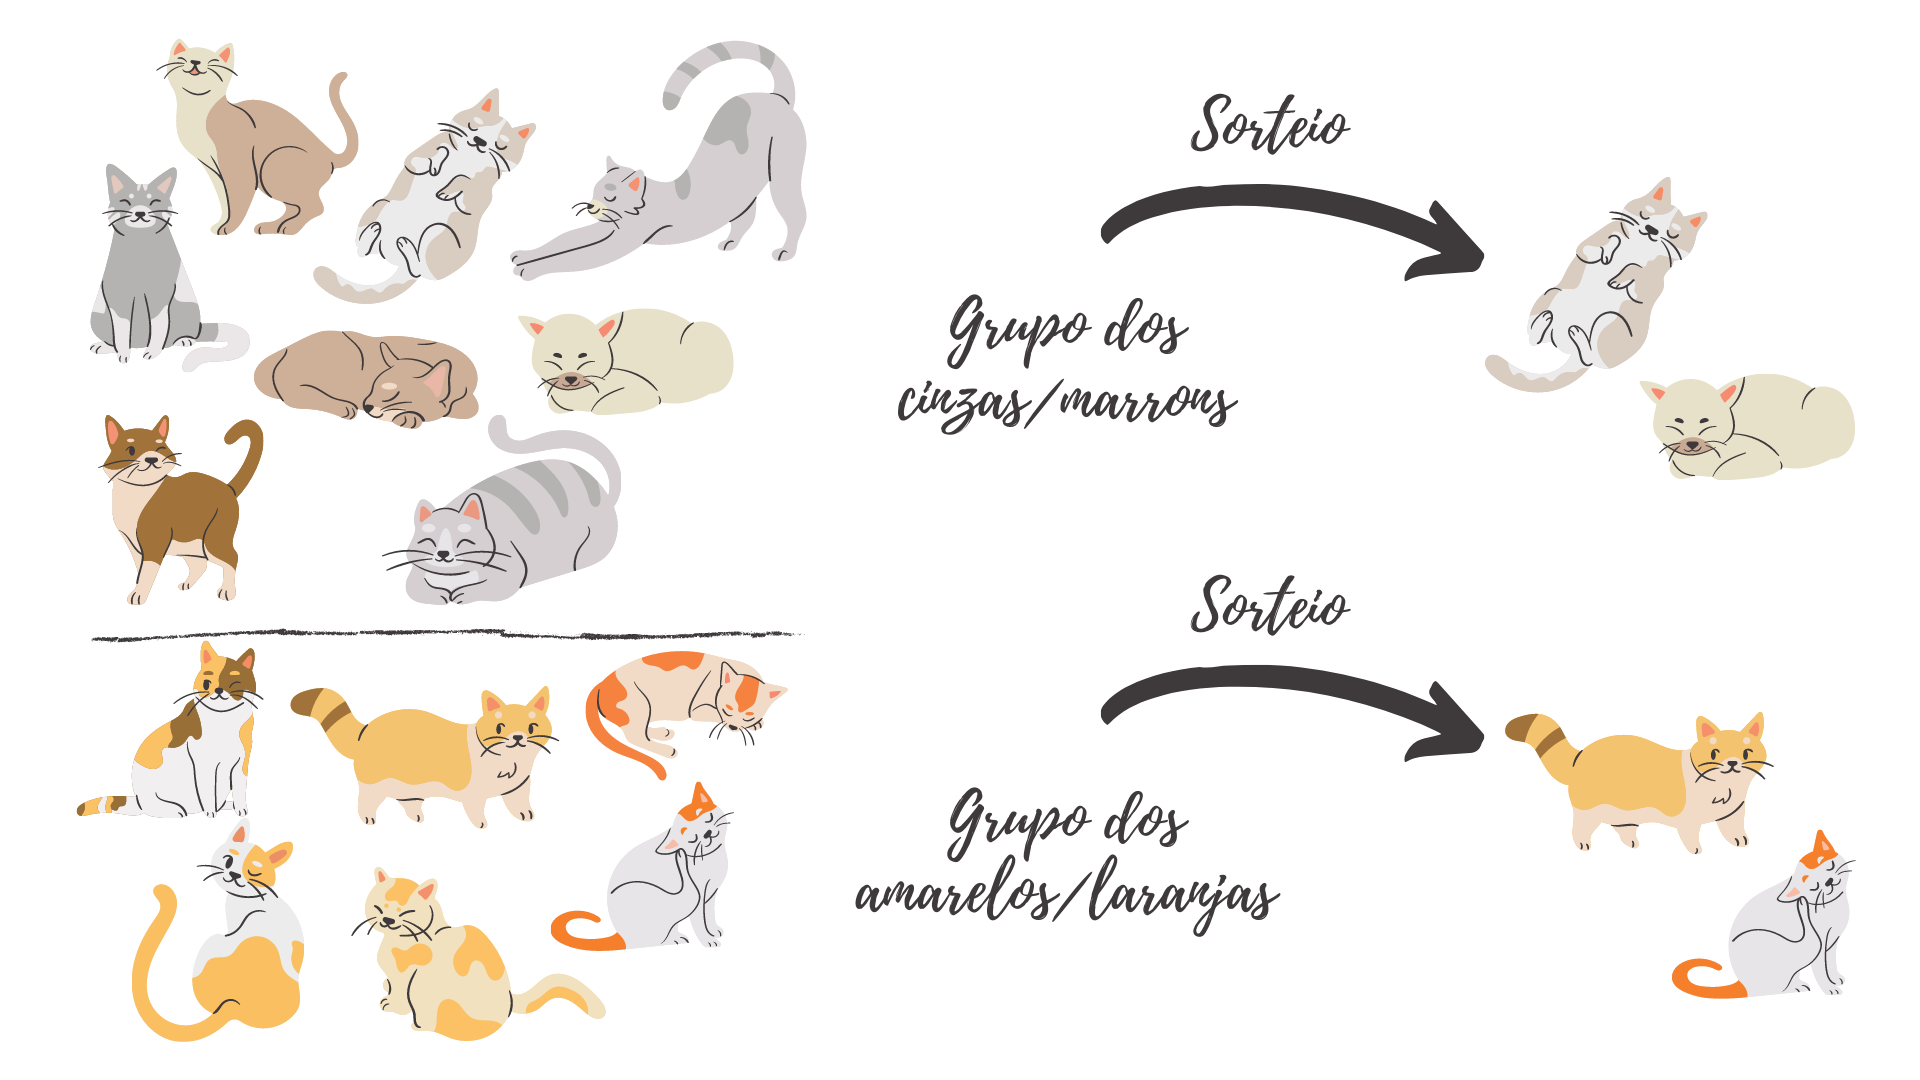
\includegraphics[scale=0.25]{figures/estratificada1.png}
    \caption{Exemplo de Amostragem Estratificada Geral.} 
    \textbf{Fonte}: leticia.raposo@uniriotec.br 
    \label{fig:amostragem_estratificada}
\end{figure}

\newpage
A estratificação uniforme é recomendável se os estratos populacionais tiverem tamanhos aproximados. Caso contrário, a proporcional é preferível por fornecer uma amostra mais representativa. 
\vskip0.3cm

É importante observar que a precisão da amostra não depende unicamente da dimensão da população, mas também da sua variabilidade. Um estrato com maior variância (maior heterogeneidade interna) deve levar à seleção de um número maior de unidades amostrais quando comparado a um estrato de mesma dimensão, porém mais homogêneo. Esse método é conhecido como \textbf{distribuição estratificada otimizada}.
\vskip0.3cm

Para calcular o tamanho da amostra estratificada proporcional para cada estrato $h$, utiliza-se a fórmula (QUEIROZ, 2012):

\begin{equation}\label{amostestra}
n_{h} = n \times \left( \frac{N_{h}}{N} \right)
\end{equation}

Onde:
\begin{itemize}
    \item $N$: número total de unidades da população;
    \item $N_{h}$: número de unidades no estrato $h$;
    \item $n$: tamanho total da amostra (soma de todos os estratos);
    \item $n_{h}$: tamanho da amostra a ser medida no estrato $h$.
\end{itemize}

Determinadas populações finitas podem ser tratadas como infinitas caso o tamanho da amostra não exceda 5\% da população:
\begin{enumerate}
    \item Se $\frac{N_h - n_h}{N_h} \geq 0,95$, a população é definida como \textbf{Infinita};
    \item Se $\frac{N_h - n_h}{N_h} < 0,95$, a população é definida como \textbf{Finita};
    \item O termo $\frac{N_h - n_h}{N_h}$ é o fator de \textbf{correção para população finita}.
\end{enumerate}
\vskip0.3cm


\newpage
\textbf{Exemplo Prático: Estudo sobre Agressão Sexual (Pará)}
\vskip0.3cm

Castro et al. (2016) realizou um estudo com base em processos judiciais de agressão sexual contra crianças e adolescentes (2012-2014) em três municípios paraenses: Abaetetuba, Belém e Parauapebas. 


\begin{table}[!htb]
    \centering
    \caption{Processos judiciais julgados pelo TJE-PA (2012 a 2014).}
    \label{tab:processos_para}
    \vspace{0.2cm}
    \begin{tabular}{l|c|c}
    \hline\hline
    \textbf{Municípios} & \textbf{N\º de Processos ($N_h$)} & \textbf{Percentual} \\
    \hline\hline
    Abaetetuba   & 47   & 6,9\%   \\
    Belém        & 555  & 82,3\%  \\
    Parauapebas  & 73   & 10,8\%  \\
    \hline
    \textbf{Total (N)} & \textbf{675} & \textbf{100,0\%} \\
    \hline\hline
    \end{tabular}
\end{table}

Devido a restrições de acesso e ao volume dos processos físicos, optou-se por uma amostra representativa com erro de 5\% ($\epsilon_0 = 0,05$). O cálculo inicial resultou em $n = 251$ processos. 

Para manter a proporcionalidade municipal, aplicou-se a técnica estratificada:
\begin{itemize}
    \item \textbf{Abaetetuba ($n_{h1}$):} $251 \times (47/675) = \mathbf{18}$ processos.
    \item \textbf{Belém ($n_{h2}$):} $251 \times (555/675) = \mathbf{206}$ processos.
    \item \textbf{Parauapebas ($n_{h3}$):} $251 \times (73/675) = \mathbf{27}$ processos.
\end{itemize}

O total amostral final é de \textbf{251 processos}, distribuídos de forma a respeitar a realidade de cada município estudado.
%----------------------------------------------------------------------------------------%




%----------------------------------------------------------------------------------------%
\subsection{Amostragem Sistemática (AS)}

A amostragem sistemática consiste em sortear uma unidade da população e, a partir dela, para constituir
uma amostra de tamanho n, selecionar as unidades que ocupam de forma sequencial as suposições multiplas
de um determinado valor $k=\frac{N}{n}$ pré-estabelecido, onde N é o número de unidades total da população (QUEIROZ, 2012).\vskip0.3cm

No processo de amostragem sistemática a primeira unidade é escolhida ao acaso e as demais, a partir da inicial, selecionadas de modo sistemático a intervalos iguais e definidas, até atingir o tamanho da amostra desejada. O intervalo é estabelecido pela razão entre o tamanho da população e o tamanho da amostran (AYRES, 2010).\vskip0.3cm

De acordo com Loetsch et al (1973) a amostragem sistemática consiste em selecionar unidade de amostras a partir
de um esquema rígido e preestabelecido de sistematização segundo uma distribuição espacial equitativa ou mecânica, com os propósitos de cobrir a população em toda a sua extensão, e obter um modelo sistemático simples e uniforme. \vskip0.3cm


\begin{figure}[H]
    \centering
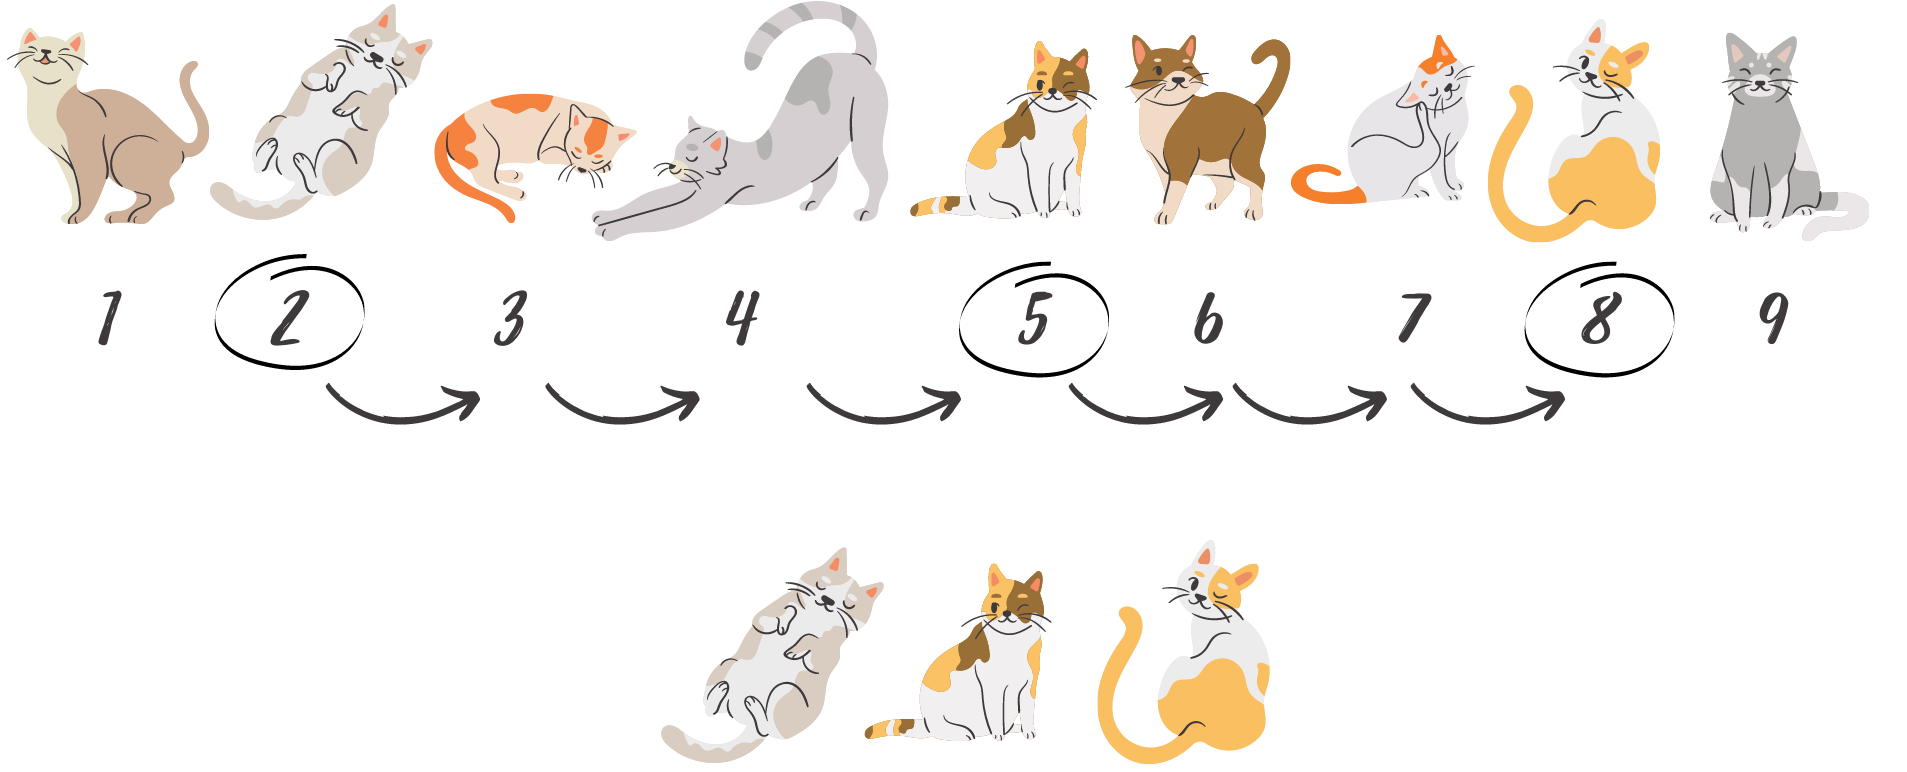
\includegraphics[scale=0.26]{figures/sistematica1.png}
    \caption{Exemplo de Amostragem Sistemática Geral.}
    \label{fig:amostragem_estratificada}
\end{figure}



A amostragem sistemática apresenta uma diferença marcante com relação a amostragem aleatória simples, no que tange
ao número de amostras possíveis. Sendo recomendada para utilização quando os elementos da população encontram-se
ordenados (MARQUES, 2002).\vskip0.3cm

Seja uma população composta por N unidades, e n represente o tamanho da amostra, sendo $N=kn$. Se a amostragem for sistematica, o número de amostras possíveis é igual a $k =\left[ \frac{N}{n} \right] $, enquanto que, em se tratando de uma amostra simples ao acaso sem reposição, o número de amostras possíveis (nap) será de acordo com a equação \ref{nap}. Então, teoricamente, uma amostra sistemática não pode ser analisada como se fosse uma amostra aleatória simples. \vskip0.3cm

De forma geral, na amostragem sistematica, utiliza-se a ordenação
natural dos elementos da população (prontuários, casas, ordem de
nascimento, etc), considerando N o tamanho da população e n o
tamanho da amostra, calcular o intervalo de amostragem, ou o pulo
sistematico, chamado k, por meio da formula $k=\frac{N}{n}$, senfo
k um numero inteiro mais proximo.\vskip0.3cm

Posteriormente, sorteia-se um numero entre um e k, chamado i,
sendo $0 < i \leq k$. Esse numero i será o primeiro elemento da
amostra. O segundo elemento da amostra será $i+k$, o terceiro
elemento será $i+2k$, e assim sucessivamente, de forma sistematica
até $i+(n-1)k$, ou seja, até completar o valor de n.


\textbf{Vantagens da Amostragem Sistemática}
\vskip0.3cm

A amostragem sistemática, quando comparada com a amostra simples, apresenta algumas vantagens, entre as quais:

\begin{enumerate}
  \item[{a)}] A seleção das unidades amostrais, na amostragem sistemática, é mais fácil e mais rápida, economizando tempo na obtenção dos dados de campo;
  \item[{b)}] A organização, a supervisão e a checagem (remedição) de algumas unidades de amostras se tornam operacioanalmente mais fáceis;
  \item[{c)}] O tamanho da população não precisa, necessariamente, ser conhecido;
  \item[{d)}] A redução de custo ocasionados pelo encaminhamento entre as unidades de amostras;
  \item[{e)}] As unidades se distribuem mais uniformemte na população, originalmente uma maior representatividade, tornando-se eficiente quando existe qualquer tendência ou concentração de certas características;
  \item[{f)}] È possível mapear a população;
  \item[{g)}] A amostragem sistemática pode ser associada  a amostragem por conglomerado;
\end{enumerate}

\textbf{Desvantagens da Amostragem Sistemática}
\vskip0.3cm

\begin{enumerate}
  \item[{a)}] A grande desvantagem da amostra sistematica ocorre
  quando a população apresenta dados com características \textbf{cíclicas}
  \textbf{ou periódicas}, pois corre-se o risco da amostragem refletir
  homogeneidade numa condição sabidamente heterogênea;
  \item[{b)}] Escolhe-se somente uma unidade de amostra simples, as demais não são independentes (estatisticamente, cada unidade não corresponde a um grau de liberdade). Assim, a variância da amostra e a da média não podem ser calculados através dos estimadores usuais;
  \item[{c)}] Escolhidos as amostras sistematicamente, todas as outras uniadades de amostra que não a integram têm probabilidade igual a zero de serem eleitas, enquanto as que integram-na possuem probabilidade 1 de seleção, ou seja, muitas unidades de amostras são, nesse caso, rejeitadas;
\end{enumerate}

\textbf{Exemplo de Amostragem Sistemática}
\vskip0.3cm

Retomando-se o exemplo de Castro et al (2016), ao qual calculou-se o tamanho da amostra estratificada porporcional por municípios, ao fazer o levantamento deparou-se com elementos da população em forma de pilhas de processos judiciais ordenados e sequenciais. Havendo assim, a necessidade de se aplicar o Método de Amostragem Sistemático para se mapear a população de forma fácil e rápida.\vskip0.3cm


\begin{table}[!htb]
    \centering
    {
    \caption{Amostragem de Processos judiciais sobre práticas de agressão sexual com criancas e
adolescentes julgados pelo TJE em três municípios Paraenses no período de 2012 a 2014.}
    \label{amostras estratificada}
    \vspace{0.1cm}
\begin{tabular}{c|c|c}
  \hline\hline
  Municípios   & Nº de Processos &  Percentual \\
  \hline\hline
   Abaetetuba  & $N_{(h1)}=47$     & $n_{(h1)}= 6.69$        \\
   Belém       & $N_{(h2)}=555$    & $n_{(h2)}= 82,22$       \\
   Parauapebas & $N_{(h3)}=73$     & $n_{(h3)}= 10,81$       \\
   \hline\hline 
   Total       & $N_{(Total)}=675$ & $n_{(total)}=251$ \\ 
  \hline\hline
\end{tabular}}
\\
\hspace{-1.0cm}
\end{table}


%\vskip0.3cm

A amostragem sistemática consiste em selecionar unidade de amostras a partir
de um esquema rígido e preestabelecido de sistematização segundo uma distribuição
espacial equitativa ou mecânica, com os propósitos de cobrir a população em toda
a sua extensão, e obter um modelo sistemático simples e uniforme.\vskip0.3cm

De forma geral, na amostragem sistemática, utiliza-se a ordenação natural dos elementos da população (nesse caso os processos judiciais de agressores sexuais), considerando N o tamanho da população (675) e n o tamanho da amostra (251), calcular o intervalo de amostragem, ou o pulo sistemático, chamado k, por meio da fórmula abaixo,

\begin{equation}
K= \left[ \frac{N}{n} \right]= \left[ \frac{675}{251} \right] = 3
\end{equation}

\newpage
Posteriormente, sorteia-se um número entre 1 e k=3, chamado i, sendo que esse número i serão o primeiro elemento da amostra. O segundo elemento da amostra será (i+3), o terceiro elemento será (i+2)3, e assim sucessivamente, de forma sistemática até i(n-1)3, ou seja, ate completar o valor de amostra n=251.\vskip0.3cm

Assim calcula-se o k, verifica-se que sorteando um número entre 1 e k=3, tem-se o número i=2, assim, a amostra ficará da seguinte maneira:




\begin{table}[!htb]
    \centering
    {
    \caption{Amostragem sistemática sobre práticas de agressão sexual com crianças e adolescentes julgados pelo TJE em três municípios Paraenses no período de 2012 a 2014.}
    \label{amostras estratificada}
    \vspace{0.1cm}
\begin{tabular}{c|c|c|c|c|c|c|c|c|c}
  \hline\hline
   2  & 5  & 7  & 10 & 13 & 15 & 18 & 21 & 24 & 26 \\
   29 & 32 & 34 & 37 & 40 & 42 & 45 & 48 & 50 & 53 \\
   56 & 58 & 61 & 64 & 67 & ... & ... & ... & ... & 674 \\
  \hline\hline
\end{tabular}}
\\
\hspace{-1.0cm}
\end{table}



\subsection{Amostragem Por Conglomerados ou Clusters}

A amostragem por conglomerados ou grupos é uma variação de qualquer processo de amostragem que, em vez de utilizar unidades de amostras individuais, usa um grupo ou conglomerado de pequenas subparcelas ou unidades secundárias (QUEIROZ, 2012).\vskip0.3cm


\begin{table}[!htb]
\centering
    {
    \caption{Esquema Geral sobre Amostragem por Conglomerados}
    \label{amostras estratificada}
    \vspace{0.1cm}
\begin{tabular}{c|c|c|c|c|c}
\hline\hline
\multirow{2}{*}{Subparcelas} & \multicolumn{5}{c}{Conglomerados}              \\
\cline{2-6}
                             & 1         & 2        &   3       & $\cdots$ & N            \\
\hline\hline
1                            & $y_{11}$  & $y_{21}$ &  $y_{31}$ & $\cdots$ & $y_{N_{1}}$  \\
2                            & $y_{12}$  & $y_{22}$ &  $y_{33}$ & $\cdots$ & $y_{N_{2}}$  \\
...                          & $\cdots$  & $\cdots$ &  $\cdots$ & $\cdots$ & $\cdots$     \\
M                            & $y_{1M}$  & $y_{2M}$ &  $y_{3M}$ & $\cdots$ & $y_{N_{M}}$   \\
\hline\hline
Totais                       &  $y_{1.}$ & $y_{2.}$ &  $y_{3.}$ &   $\cdots$       & $y_{N.}$   \\
\hline\hline
\end{tabular}}
\end{table}

Apesar de a amostragem estratificada apresentar resultados
satisfatórios, a sua implementação é dificultada pela falta
de informações sobre a população para fazer a estratificação.



Para poder contornar esse problema, pode-se trabalhar com o
esquema de levantamento chamado amostragem por conglomerados.\vskip0.3cm

Os conglomerados são definidos em razão da experiência
do gestor ou do pesquisador. Geralmente, podemos definir os
conglomerados por fatores geográficos, como bairros e quarteirões.
A utilização da amostragem por conglomerados possibilita uma
redução significativa do custo no processo de amostragem.\vskip0.3cm

A amostragem por conglomerados ou também chamada de clusters, é usada quando a população
pode ser dividida em subpopulações heterogêneas.\vskip0.3cm


Uma amostragem por conglomerado é indicada quando:

\begin{itemize}
  \item Não se possui uma lista contendo todos os nomes dos elementos da população;
  \item Existe grande heterogeneidade entre os elementos da população-alvo;
  \item É preciso fazer entrevistas ou observações em grandes áreas geográficas;
\end{itemize}



\begin{figure}
    \centering
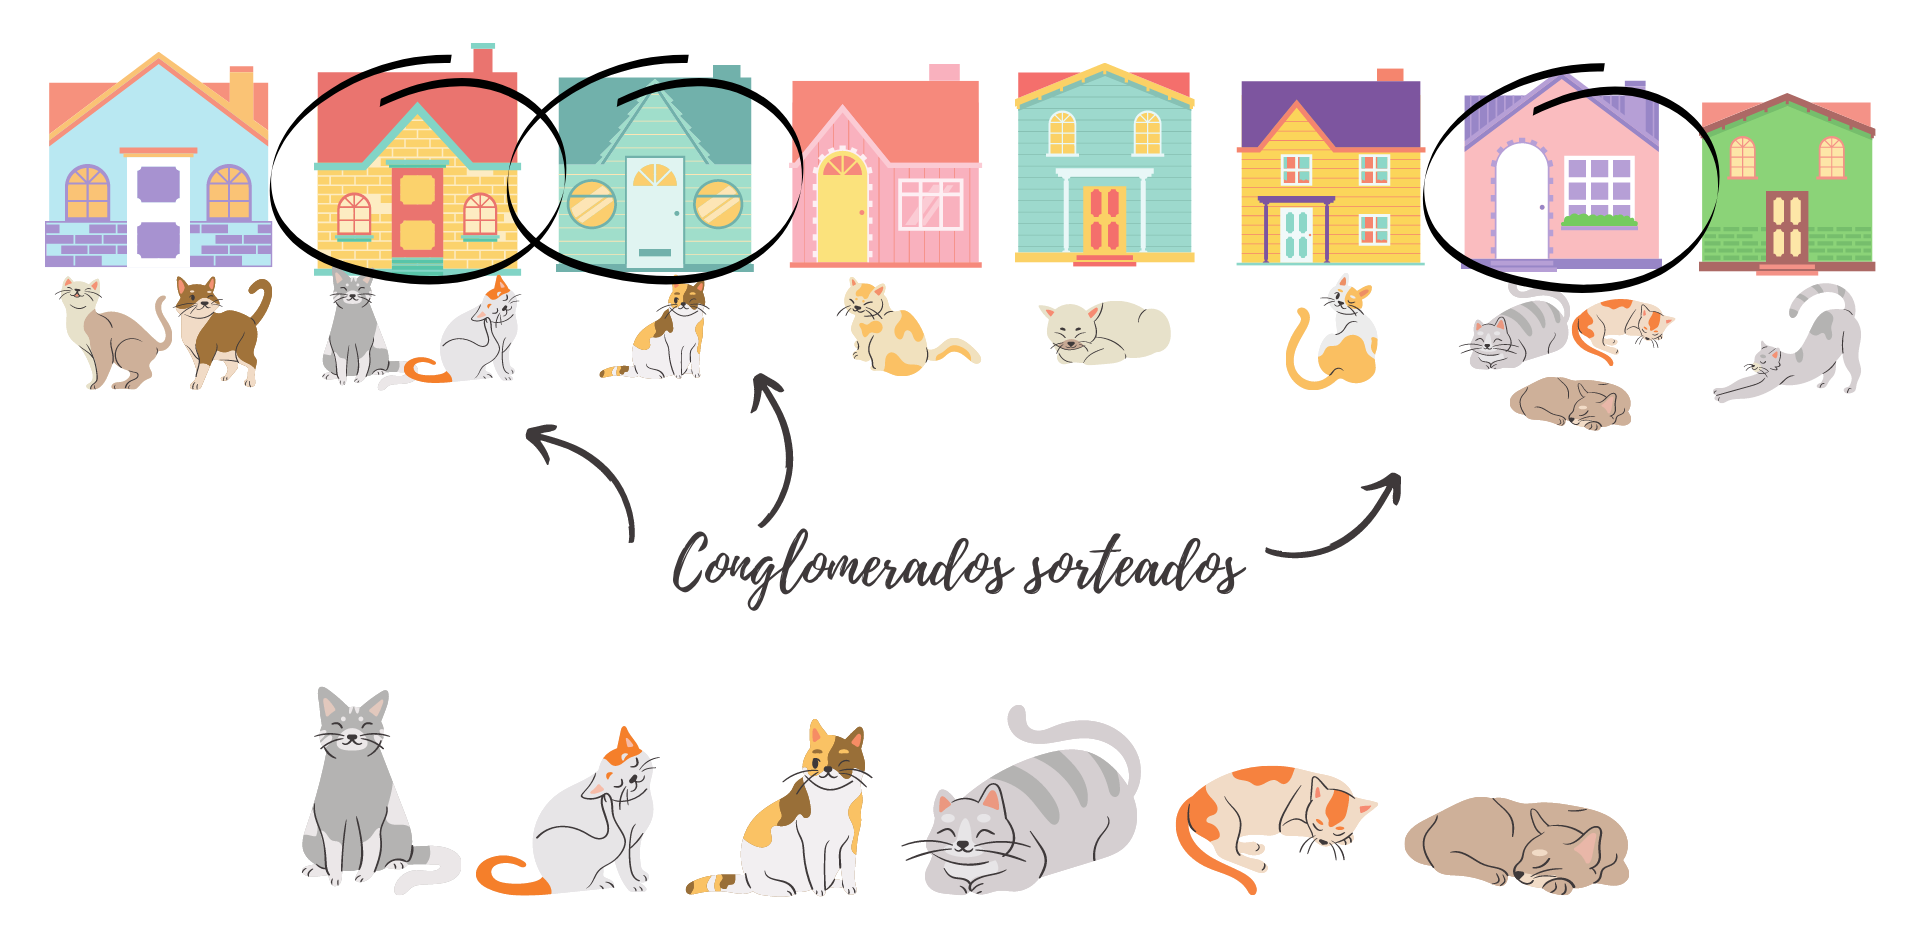
\includegraphics[scale=0.25]{figures/cluster1.png}
    \caption{Exemplo de Amostragem por Conglomerado Geral.}
    \label{fig:my_labe21}
\end{figure}





\newpage
As unidades de amostragem ou grupos podem ser espaçadas como ocorre naturalmente em unidades geográficas ou físicas (por exemplo, estados, delegações ou distritos); em base  a uma organização como escolas, grau escolar; ou serviço telefônico, tais como códigos de área ou alterar o código de área do serviço dos números de telefone.\vskip0.3cm

Duas grandes dimensões são utilizadas para classificar os diferentes tipos de amostragem por conglomerados. Uma baseia-se no número de fases do projeto da amostra, e o outra na representação proporcional de grupos na amostra total.\vskip0.3cm


A principal Desvantagem dos cluters é que, os conglomerados raramente são do mesmo tamanho, dificultando o controle da amplitude da amostra. Além disso, pode introduzir maior variabilidade nos resultados, já que os elementos dentro de cada conglomerado tendem a ser mais semelhantes entre si, aumentando o erro amostral.



\newpage
\section{Amostragem Não Probabilística}

Os métodos de amostragem não probabilística, dirigido ou também chamados de não aleatória, são métodos ad-hoc de caracter pragmático ou intuitivo e são largamente utilizados, pois possibilitam um
estudo mais rápido e com menores custos.


\subsection{Amostragem por Conveniência ou Acidental}

A amostragem por conveniência ou acidental é uma técnica não probabilística, amplamente utilizada em pesquisas exploratórias devido à sua simplicidade, rapidez e baixo custo. Apesar de ser útil em situações específicas, ela possui limitações importantes, principalmente relacionadas à falta de representatividade da população.\vskip0.3cm

As pricipais características sobre Amostragem por Conveniência são:

\begin{itemize}
    \item \textbf{Rapidez e Facilidade}: Utiliza unidades acessíveis ou disponíveis no momento da pesquisa, como grupos próximos do pesquisador.
    \item \textbf{Baixo Custo}: É uma opção econômica, pois dispensa processos elaborados de seleção.
    \item \textbf{Aplicações Frequentes}: Estudos exploratórios para geração de ideias iniciais. Pré-testes de questionários ou instrumentos de pesquisa. Pesquisas com limitações de tempo ou orçamento.
    \item \textbf{Baixa Confiabilidade}: A seleção das unidades depende do critério do pesquisador, o que pode introduzir vieses significativos. Não há garantias de que os resultados sejam representativos da população estudada.
    \item \textbf{Quando Utilizar}: Pré-testes de questionários, Estudos exploratórios ou pilotos, e Pesquisas rápidas ou de baixo custo, quando a representatividade não é a prioridade.
\end{itemize}



\newpage
\subsection{Amostragem Intencional ou por Julgamento}

A amostragem intencional ou por julgamento é uma técnica de amostragem não probabilística em que o pesquisador utiliza seu conhecimento, experiência ou critérios específicos para selecionar os elementos que ele acredita serem mais representativos ou relevantes para o estudo. Aqui estão os principais aspectos e exemplos para ilustrar sua aplicação:

\begin{itemize}
    \item \textbf{Critério Baseado no Conhecimento}: A escolha dos elementos é feita com base no julgamento do pesquisador, que identifica indivíduos, locais ou grupos considerados mais adequados para o objetivo da pesquisa;
    \item \textbf{Representatividade Percebida}: A abordagem se baseia na premissa de que os elementos escolhidos são "típicos" ou "representativos" do fenômeno estudado;
    \item \textbf{Tamanho da Amostra}: Essa técnica é frequentemente usada quando o tamanho da amostra é pequeno e o pesquisador precisa otimizar a seleção para maximizar a relevância dos dados;
    \item \textbf{Aplicações Comuns}: Seleção de especialistas para estudos qualitativos. Escolha de localidades "modelo" para entender fenômenos mais amplos. Estudos iniciais ou exploratórios em que se busca profundidade em vez de amplitude;
    \item \textbf{Vantagens}: Simplicidade e rapidez na seleção.
Foco em elementos-chave que podem gerar insights valiosos;
Útil quando o pesquisador possui amplo conhecimento do contexto
    \item \textbf{Limitações}: Alto risco de viés, pois depende da subjetividade do pesquisador.
Pode não ser representativo de toda a população, comprometendo a generalização dos resultados.
\end{itemize}

Essa abordagem, embora limitada na representatividade estatística, pode fornecer informações valiosas e detalhadas para a compreensão de fenômenos complexos, como os relacionados ao trânsito.

\newpage
\subsection{Amostragem por Quotas ou Proporcional}

A amostragem por quotas ou proporcional é uma abordagem muito utilizada em pesquisas quando o objetivo é garantir que a amostra reflita, de maneira aproximada, as características da população em estudo. Aqui estão os pontos mais relevantes sobre este método:


\begin{itemize}
    \item \textbf{Definição e Objetivo}:
A amostragem por quotas é um tipo de amostragem não probabilística em que o pesquisador busca obter uma amostra semelhante à população com base em características específicas, como gênero, idade, raça ou renda. Isso é feito para assegurar que a amostra represente a diversidade da população em relação a essas variáveis;
\item \textbf{Processo de Seleção}: Primeiro, são identificadas as características relevantes da população que precisam estar representadas na amostra. Em seguida, calcula-se a proporção de cada grupo na população. Com base nessas proporções, o pesquisador estabelece quotas (número de participantes por grupo) que devem ser preenchidas;
\item \textbf{Instruções aos Entrevistadores}:
Os entrevistadores são orientados a buscar pessoas que se encaixem nas características definidas até que a quota de cada grupo seja atingida.
\item \textbf{Vantagens}: É um método rápido e de baixo custo, já que dispensa a necessidade de uma seleção aleatória complexa. Permite um controle maior sobre as características da amostra, assegurando que ela seja representativa em aspectos relevantes. Útil quando as características populacionais são bem conhecidas e estão relacionadas ao objeto de estudo.
\item \textbf{Limitações}: Não garante representatividade probabilística, uma vez que os participantes são selecionados de forma intencional, e não aleatória. A qualidade dos resultados depende da habilidade e do julgamento do entrevistador, podendo haver viés de seleção. Pode ser inadequado quando as categorias relevantes para a pesquisa são numerosas ou difíceis de identificar.
\end{itemize}

A amostragem por quotas é amplamente utilizada em pesquisas de mercado, pesquisas sociais e políticas, onde a rapidez e a flexibilidade na coleta de dados são fatores importantes.